% \part{\VV Methods and Tools }
% \label{sec:methods-tools}

The project shall select / develop / describe a chain of methods and
tools for doing \vv in a full development. In Version V01, this
section collects proposals, which will be evaluated and from which
those suitable for real-life
development and maintenance of the open-source EVC software will be selected.

Each proposal described here shall be classified for which tasks and
activities in teh development it is intended, i.e., which role it
should take.

\bgcmmnt{A common format should be included, adressing:
  \begin{description}
  \item[Contributor] Person or organisation who contributed the
    description. Should name a contact for further information
    concerning the method or tool. In case of modifications or
    additions by others than the contributing party, these others
    shall be added.
  \item[Purpose] For which activites this method/tools might be useful
  \item[Evaluation/Evidence] Has it been demonstrated somehow?
    Summary, pointers, etc.
  \item[Review] Has the evidence been assessed (internal asssessment, verdict)?
  \item[Tool qualification] Needs/done/Ideas
  \end{description}
}

\chapter{On the Notion of ``Formal Methods''}
\label{sec:notion-formal-method}

As FLOSS relies to a large extent on the use of tools for generating, 
verifying and validating a design, ``formal methods'' necessarily will
play an important role in the openETCS activities.  

In common language, the notion {\em ``formal''} is often used in a
broad sense, meaning everything that can be described by rules, even
if they are rather vague.
%
Contrary to that, we use {\em ``formal''} in the narrow sense of
EN-50128 \cite[Section~D.28]{en50128},
meaning strictly mathematical techniques and methods.
%
Since the Aerospace Standard DO-178C \cite{DO-178C}
follows a similar understanding,
but gives more elaborate explanation in its supplementary document
%DO-333 
devoted to formal methods \cite{DO-333},
our presentation closely follows the terminology of the latter.


\begin{quote}
{\em Formal methods are mathematically based techniques for the
specification, development, and verification of software aspects of
digital systems.
%
The mathematical basis of formal methods consists
of formal logic, discrete mathematics, and computer-readable
languages.
%
The use of formal methods is motivated by the expectation
that, as in other engineering disciplines, performing appropriate
mathematical analyses can contribute to establishing the correctness
and robustness of a design.}

\hfill
\cite[Section~1.0, p.1]{DO-333}
\end{quote}


\chapter{Reviews and Inspections}
\label{sec:reviews-inspec}

Not everything can be done by formal methods. The introduction of reviews
 in the openETCS project will enable the
adherence to design specifications as well as ensuring that
appropriate coding techniques---for automatic generation as well as 
observation of relevant coding
standards---have been used.  The use of an appropriate review technique
will also help to ensure the consistency of approaches across development teams
and may result in improved standards through the identification of
best practice solutions.  Software reliability will be increased due
to the removal of a larger percentage of the errors that would
otherwise remain in the software. Specific analysis techniques
exist for predicting the reliability of software.

For verifying any product, whether it is a piece of
software, a design specification, test script or anything else, it is 
essential to carry out some sort of review or inspection process. 
The introduction of formal review processes provides us with 
definite points in time when we can carry out these essential 
assessments.

It is possible to review just about anything. In the openETCS project
all written documents, specifications, models and code can be
reviewed. It is also important to include all documents concerned with
the creation and delivery of the openETCS product. This means that
strategies, plans, approaches, operation and maintenance manual, user
guides, the contract that will initiate the work should all be
reviewed in a structured way.

\paragraph{Inspection}
On the other hand, an inspection is a visual examination of a software
product to detect and identify software anomalies, including errors
and deviations from standards and specifications
\cite{Fag76-99}. Inspections are peer examinations led by impartial
facilitators who are trained in inspection techniques. Determination
of remedial or investigative action for an anomaly is a mandatory
element of a software inspection, although the solution should not be
determined in the inspection meeting.

Both review and inspection methods shall be used in different
contexts during the execution of the Verification activities.

More information about the reviews can be found in Quality Assurance Plan
\cite{QAplan}.

\chapter{Software Architecture Analysis Method (SAAM)}

SAAM \cite{KABC96} is one of the simpler methods for a scenario-based
architecture evaluation, and it was the first to be published. SAAM is
suitable for the testing of software architectures with regard to
quality attributes (qualitative requirements), such as
%
\begin{itemize}
\item Modifiability,
\item Portability,
\item Growth Potential,
\item Performance,
\item Reliability,
\end{itemize}
%
but also for the evaluation of the functionality (functional 
requirements) of a software architecture. 

In a SAAM evaluation basically scenarios are developed, 
prioritized and assigned to those parts of the software 
architecture to be tested that are affected by them. 
This may be sufficient to indicate problems in the architecture.

\chapter{Architecture Tradeoff Analysis Method (ATAM)}	
\label{sec:atam}

ATAM \cite{ATAM} is used to review the design decisions of the architecture. 
It is checked whether the design decisions satisfactorily 
support the requirements concerning quality. Risks and 
compromises included in the architecture are identified 
and documented.

The process includes two phases. 
\begin{itemize}
\item In the first phase the necessary components 
	are presented. Then the architecture is checked and analyzed. 
\item In the second phase it is tested whether the analysis 
	and the test were correct and complete. Then the 
	results are summed up.
\end{itemize}

\chapter{Model Based Testing Method}
\label{subsec:mbt}
\section{Model Based Testing Strategy - generalities}
Testing consists in executing the System Under Test (SUT) for some
particular inputs and in assessing whether or not the corresponding
SUT executions conform to some requirements.  Whatever the testing
technique used is, one has to define test cases to be submitted to the
SUT and associate to them a decision procedure called oracle. The
oracle allows the tester to compute verdicts according to what the
executions of SUT (resulting from the test case submission) reveal
about its correctness.  This correctness is measured with respect to
requirements. Model based testing is a particular kind of testing
technique in which requirements are described by models which are
executable specifications. Their execution traces (or ``traces'' for
short) are sequences of stimulations of the SUT and resulting
observations of the SUT reactions. Test cases are sequences of
stimulations that are selected from the test model. A sequence
corresponding to an input test data can be obtained by considering a
trace of the model and ``forgetting'' it. For functional testing, SUT
is considered as a black bbox: the tester (a human or a test bench)
can only stimulate the SUT and observe its reactions. Interactions
between the tester and the SUT result on the definition of
traces. Therefore, a SUT can be seen as a set of traces that is not
known (since SUT is a black box) but the tester may discover some of
those traces by interacting with SUT. The oracle is based on a so
called conformance relation. A conformance relation is a mathematical
relation between the set of traces of the SUT and the set of traces of
the model.  When these sets of traces fulfill the relation we say that
the SUT conforms to the model. The oracle takes as inputs traces
representing an interaction between the tester and the SUT and compute
verdicts. Whatever the testing technique is, the set of possible
verdicts always contain the verdict Fail which is emitted whenever the
trace taken as input demonstrates that the SUT does not conform to the
model. Depending on the testing technique used there may be different
verdicts emitted when Fail is not emitted. These different verdicts
reflect different traceability information related to interaction
trace taken as input. In this section we briefly discuss two model
based testing tools that we will use conjointly in the OpenETCS
project.

Model based testing (MBT) may apply at different level during the
lifecycle:
\begin{itemize}
\item System integration testing
\item Software integration testing
\item High level code verification
\item Object code verification
\end{itemize}
High-level code verification may be performed on any host perform
whereas object code verification intends to test the running code on
the target hardware.

\paragraph{Model-Based System Integration Testing}
The objectives of MBT on system integration level are to
\begin{itemize}
\item validate the correctness and completeness of the development model,
\item verify that the generated code components cooperate correctly on
  the target HW, in order to achieve the system-level capabilities.
\end{itemize}

The first objective implies that the {\it test model} and the original
development model are separate entities; otherwise the system
integration test would just validate that all logical errors still
residing in the openETCS development model are really implemented in
the code. Even in presence of a formally validated development model,
in which high confidence can be placed, we prefer to create a separate
test model, because
\begin{itemize}
\item the test model may use a higher level of abstraction since only
  the SUT behaviour visible at the system interfaces is relevant,

\item the test model may specify different interfaces to the SUT,
  depending on the observable interfaces in a test suite; the
  observation level ranges from black-box (only the ``real'' SUT
  system interfaces are visible) to grey-box level (some global
  variables may be monitored or even manipulated by the testing
  environment, some task or object communications may be observed
  etc.),

\item the development model may contain errors that are only revealed
  during HW/SW integration (for example, calculations failing due to
  inadequate register word size, or deadlines missed due to
  insufficient CPU resources).
\end{itemize}

Software integration is performed by software-in-the-loop technology
on host computers. The software components as well as the complete
software are tested on host computer with a testing environment that
simulates the hardware behavior and the operational environment. The
main advantage is that all software properties can be easily simulated
and tested. The tests for software-in-the-loop may be generated from a
model but at this level unite test for each software functionalities
may also be performed.

\paragraph{Model-Based Testing of Generated High-Level Code}
Another application of MBT aims at the verification of generated
high-level code (for openETCS, the target language will be C).  If
model-to-text transformations are not formally verified, it is
necessary to verify the outcome of each transformation. Since the
transformation source is a model $M$, MBT suites can be derived
automatically from this model to show that the generated code conforms
to $M$.

Observe that in contrast to system-level MBT no redundant model is
used for this objective, but the same model $M$ used for code
generation can be used: we just have to verify the consistency between
code and $M$, without validating $M$'s correctness and
completeness. The latter task is separately performed by means of
\begin{itemize}
\item property checking or
\item simulation.
\end{itemize}
The model-based testing (MBT) approach can be used to create test
suites conforming to the highest criticality level of the applicable
CENELEC standards, in order to justify that the generated code is
consistent to its model~\cite{PeleskaVL11Nfm,pel2011a,peleska2009d}.
Furthermore, the generated result may be formally verified against the
model. This formal verification task is easier than proving the
correctness of a generator or compiler as a whole, because now just
one concrete artefact (the generated code) has to be checked against
the transformation source. The theoretical foundations of object code
verification, as well as its proof of concept have been established
in~\cite{Pnueli98}. In
\cite{RSRSChapter2012,DBLP:journals/fac/HaxthausenPK11} these concepts
have been refined and applied to the railway domain.


The  main advantage of this approach in comparison to performing V\&V for
generators and compilers is that the latter do not have to be
re-verified after improvements and extensions. Therefore we advocate
the test-based code verification approach to be applied in openETCS
for verifying generated high-level source code or object code of SIL-4
applications. 


The HW/SW integration testing is out of the scope of this
project. Nevertheless, Model-Based Testing of Compiled Object Code
or/and  Alternative Unit test on target HW may also be performed.


\section{Model Based Testing applied to Open ETCS V\&V}
According to the previous activity on defining the project process,
the Open ETCS process is based on 3 main inputs for methodology and
product lifecycle: the SCRUM methodology, the Model Driven Design and
the Cenelec software development V cycle.  Traditionally, system
requirements are directly translated into formal specifications on
which verification and proof techniques are applied. The use of formal
specifications and formal language allows then to derive the models
using dedicated languages (B for instance) in order to guaranty
conservation of properties along the design process. The main
difficulty in this context is to be sure that the interpretation of
rules has correctly been captured in the formalized specification
which is not easy to check by the regulators. For this reason, the
model based testing has been chosen as testing and verification
technique within the V\&V activities of the OpenETCS project.

Moreover, we suggest to create test models on the basis of the ETCS
standard (subset 026) and the existing high-level test suites made
available in subset 076. The latter test cases should be feasible
computations of the test model, so that the test model really creates
a {\it superset} of the existing test suite from subset 076.

This technique application will be explained in the following
paragraphs through the description of different model-based testing
tools: MaTeLo, Diversity and RT-tester.

\section{Matelo Model Based Testing solution}
MaTeLo purpose is to generate test cases for systems whose expected
usage and behavior are described by a probabilistic model. MaTeLo tool
is based on its own test model called "usage model" and uses, among
other characteristics, usage profiles for test case generation. This
usage model describes the possibilities regarding the use of the soft
(in our case; operating scenario) during its whole lifecycle. This
usage model is performed thanks to a Matelo specific modeler, it
allows to generate test cases that will then be plugged to the SUT
which will be the software semi-formal model realized in the frame of
WP3 activities.  MaTeLo has three main functionalities: test modeler,
test cases generator and test campaign analyser. Even if MaTeLo is
mainly a test case generation tool, we can consider that this tool
performs also analysis for different reasons:
\begin{itemize}
\item A test model can be considered as a development artifact the
  same way as a system model for example. So analysis on it could
  identify some ambiguous or erroneous points in test model (i.e. in
  the future test campaign) or in the specifications (because MaTeLo
  mode l is built from system specifications).
\item Even whether test campaign analysis is mainly based on testing
  activities, analysis techniques have to be used as wellThe limit
  between a model to perform test and a model to perform analysis is
  not so obvious.
\end{itemize}

Because its test case generation is based on a model, MaTeLo belongs
to the family of Model-Based Testing solutions. MaTeLo model basically
uses Markov Chains to describe the test model of the SUT implemented
for "Black Box Testing" in all xIL steps (MIL, SIL, PIL, HIL).  MaTeLo
Usage Model edition facility allows for implementing test models that
describe the use cases of the SUT completed with the tester point of
view, and then, Matelo testing facility can generate automatically the
test cases generated by the tool.  Thanks to the numerous validation
steps, MaTeLo Test Campaign Analysis provides information such as test
coverage (requirements, model) or reliability of the SUT.  Once the
MaTeLo test model is performed and the testing strategy is defined
with MaTeLo profiles faciulities, MaTeLo generates test cases. For
that, MaTeLo Testor contains several test generation algorithms that
can be used for different purposes. Different test case generators are
based on a Usage profile approach, considering the occurrence
probability of each model transition. Other are deterministic (most
probable execution path, or all the transitions are covered).  In the
case of Open ETCS project, the SUT model is an on-board EVC, designed
according to the SRS Subset 026. This specification itself is not
sufficient to cover all functional aspects, and tests depend strongly
on the operating rules to be considered on the observed track. The
principle for the MaTeLo model would be to encompass all the possible
states and transitions that can be considered in a well-defined
perimeter (based on Subset026, signaling and exploitation rules to
consider). Then, the test could be precisely defined by the usage
profile to adapt it to a track oriented testing campaign.

\section{Diversity Model Based Testing solution}
DIVERSITY is a model based testing tool developed at CEA LIST. Its
underlying technology is symbolic execution. Symbolic execution has
been first defined for programs. The goal of this technique is to
identify, for each possible execution of the program, the constraints
to be satisfied in order to follow it. The main idea consists in
executing the program, not for concrete numerical values but for
symbolic parameters, and to characterize constraints on these
parameters at each step of the execution.  In that sens, DIVERSITY is
a white box testing tool.  In the frame of the openETCS project we
plan to use DIVERSITY to extract test cases from models defined in the
first phases of the system design. Our goal is to extract test cases
dedicated to abstract safety requirements. More precisely we focus on
safety requirements dealing with communication between sub
systems. For that purpose we will use the language of sequence
diagrams extended with timing constraints to specify such
requirements. With sequence diagrams, one may describe execution
scenarios in terms of partially ordered message passing between
subsystems. Message passing can be structured thanks to operators
expressing sequencing, parallelism, choice, loop...  It is possible to
automatically analyze sequence diagrams with DIVERSITY in order to
extract test cases. The originality is that, thanks to projection
mechanisms, it is possible to extract test cases, not only for the
entire system, but also for any sub systems composing it. Because of
this mechanism, sub systems can be tested as soon as they are
implemented, even though the entire system is not yet implemented. In
such a process we perform a particular kind of unitary testing in
which unit test cases are built according to the usage that will be
made of the sub system in the entire system. In the frame of OpenETCS,
this functionality could be useful in order to realize the unitary and
modular tests.  The first step consists in defining a requirement
model in the form of a sequence diagram or a Matelo Test scenario. The
requirement model is analyzed with DIVERSITY in step 2. This analysis
results on a so-called symbolic tree, whose each path denotes a
possible (symbolic) execution of the sequence diagram. Such trees may
be theoretically infinite due to the possible occurrences of the
``loop'' operator of sequence diagrams. Therefore, DIVERSITY uses
various stopping criteria to stop the computation (typically based on
message coverage notions).  The symbolic tree computed in step 2
characterizes executions of the whole system model.  However, because
testing the whole system may be complicated in terms of testing
architecture, or simply because one wants to test some sub systems
before the whole system is implemented, we offer a mechanism to
extract symbolic trees for each distinguished sub system. This is
based on so-called projection techniques. This operation is realized
in step 3. In step 4, each identified sub system is tested thanks to a
real time off-line testing algorithm.  Then, we can relate correctness
of sub systems and correctness of the whole system by using a
compositionality theorem.  The compositionality theorem expresses
that, the conformance of each subsystems to all their projections
guarantees the conformance of the whole system to the sequence
diagram. A direct consequence is that any faults of the whole system
can be discovered as a fault of at least one of its sub systems. This
implies that testing the whole system mainly comes to test each of its
sub systems after a short test integration phase testing that each sub
system is correctly connected.  We believe that such an approach will
be very useful for ETCS systems which are by nature very distributed
and thus hardly observable and controllable as a whole. The share of
OBU EVC kernel in sub-system is the role of the SSRS model, and this
refinement to diversity will be possible once this functional
decomposition of the EVC will be released.

\section{Complementary use of the DIVERSITY and MaTeLo}
The use of the two tools can be done in a complementary way that would
allow a more efficient test case set generation.  MaTeLo would start
from the test model, and generate automatically all the use cases that
can be encountered in CBTC use. MaTeLo tool analyses the models as
black box, and generates tests according to a stochastic approach.
DIVERSITY will analyze these scenarios, based on a symbolic execution
of the semi-formal SysML model (white box testing), in order to filter
the tests generated by MaTeLo and to reduce the test case set.  As
discussed in previous Sections, the two tools DIVERSITY and MaTeLo
handle different kinds of models. The version of DIVERSITY that we
will use in the project handles high level models in the form of
sequence diagrams. Such models can be used to specify requirements on
communication scenario between subsystems of a reference system under
test. Models handled in MaTeLo are automata labeled by transfer
functions and probabilities. Such models are useful to describe
executable behaviors very close to the actual implementation, and
based on operating scenarii. Clearly these two levels of modeling are
useful in design processes of safety critical applications such as
ETCS implementations, and can be combined in different ways for
improving the test coverage of our EVC Software kernel.  Indeed, ETCS
systems have such a level of complexity, that it is difficult to
describe them in a model straight from the requirements. Therefore,
the refinements provided by two modeling levels are very
helpful. Moreover, it is mandatory to maintain a good traceability
between these two levels of modeling, in order to fulfill the safety
requirements.  The complementarity of these tools takes place in some
refinement processes in which high level requirements can be
implemented into executable models. However, it is crucial to assess
whether executable models correctly implement requirements. In
practice this may be a difficult question because it requires to
efficiently explore the executable model, which by nature is generally
huge because it represents in a precise manner the functional
behaviors of the actual implementation.  In order to overcome this
problem we plan to take benefits from the fact that executable models
of ETCS will be described in the form of communicating executable
models. This fact permits to see the model as a collection of
communicating subsystems. This permits to take benefits of the
compositional result described in the Diversity, and use it for white
box testing (the internal behavior of functional modules and blocks
defined in the kernel can then be precisely tested)..


\section{The RT-tester} 

The RT-Tester test automation tool, made by Verified
\cite{verified_website}, performs automatic test generation, test
execution and real-time test evaluation.  It supports different
testing approach such as unit testing, software integration testing
for component, hardware/software integration testing and system
integration testing.  The RT-Tester version  follows the
model-based testing approach \cite{Peleska2011} and
it provides the following features :
\begin{itemize}
\item Automated Test Case Generation 
\item Automated Test Data Generation 
\item Automated Test Procedure Generation 
\item Automated Requirement Tracing 
\item Test Management system 
\end{itemize}
Starting from a test model design with UML/SYML, the RT-tester fully
automatically generates test cases. They are then specified as test
data (sequences of stimuli with timing constraints) and used to
stimulate the SUT and run concurently with the generated test
oracles. The test procedure is the combination of the test oracles and
the SUT that can be compiled and executed.

The tool supports test cases/data generation for structural
testing. It automatically generates reach statement coverage, branch
coverage and modified condition/decision coverage (MC/DC) as far as
this is possible.  The test cases may all be linked to requirements
ensuring a complete requirement traceability.  Additionally RT-tester
may produce test cases/data from a LTL formula, since a LTL formula
describes a possible run of the model.

Taking advantage of SysML requirements diagram, the test cases and
test procedures are directly linked to the requirements. It is then
possible to perform test campaign guided by requirements.

Finally the tool may produce the documentation of tests for
certification purposes. For each test cases the following document are
produced :
\begin{itemize}
\item {\em Test procedure}: that specifies  how one test case can be
  executed, its associated test data produced and how the SUT
  reactions are evaluated against the expected results.
\item {\em Test report}: that summarizes all relevant information
  about the test execution.
\end{itemize}

In \cite{brauer_efficient_2012}, a general approach  on how to qualify
model-based testing tool according to the standard ISO 26262 ad RTCA
DO178C has been proposed and applied with success to the RT-tester
tool. Following the same  approach compatibility with the CENELEC EN50128
may be easily done. 


\chapter{Characterisation of Formal Methods}

Based on rigorous mathematical notions, formal methods may be used
to describe software systems' requirements in an unambiguous way,
thus supporting precise communication between engineers.
%
Formally specified requirements can be checked for consistency and
completeness by appropriate tools;
also, compliance between different representation levels of
specification can be verified.
%
Formal methods allow one to check software properties like:

\begin{itemize}
\item Freedom from exceptions
\item Freedom from deadlock
\item Non-interference between different levels of criticality
\item Worst case resource usage (execution time, stack, \ldots)
\item Correct synchronous or asynchronous behaviour,
        including absence of unintended behaviour
\item Absence of run-time error
\item Consistency of a formal model
\item Correctness of a formal model
\end{itemize}


In order to subsume this variety of applications under a single
paradigm,
the DO-178C
considers a formal method to consist in applying a
formal {\em analysis} to a formal {\em model}.
%
Both analysis and model differs depending on the particular method.
%
For most methods, the model
is just identical to the source code; however, it may
also be e.g.\ a tool-internally generated abstract state space (used
in the Abstract Interpretation method, cf.\
Section~\ref{sec:Abstract Interpretation} below).
%
For most methods, analysis tools need human advice;
however, they may also be fully automatic (e.g.\ for 
Abstract Interpretation or Model Checking, cf.\
\ref{sec:Model Checking}).

\chapter{Formal Analysis Methods}
\label{sec:formal-analysis}

In this section we present
the three most common methods for formal analysis.
The foundation of these analysis
methods are well understood and they have been
applied to many practical problems.


\section{Abstract Interpretation}
\label{sec:Abstract Interpretation}

The abstract interpretation method
\cite{Cousot.Cousot.1976}
builds at every point of a given program a conservative\footnote{
        i.e.\ guaranteeing soundness
}
abstraction
of the set of \emph{all} possible states that may occur there
during any execution run. Such a representation is also called an 
\emph{over-approximation}, in the sense that it captures all possible
concrete behaviours of the program, while the abstraction might lead to 
consider states that cannot occur in a concrete execution.
%
Abstract interpretation 
determines particular effects of the program relevant for the
properties to be analysed, but does not actually execute it.
%
This allows one to statically determine dynamic properties of
infinite-state programs.
%
The main application is to check the absence of runtime errors, like
e.g.\ dereferencing of null-pointers, zero-divides,
and out-of-bound array accesses.
%
While conventional ad-hoc static analysis tools such as PCLint or \mbox{QA\cxx}
are well-tailored for quick, but incomplete analyses,
abstract-interpretation based tools while requiring more computation time, are
\emph{safe} in the sense that they guarantee that {\em all} potential
runtime errors are detected. On the other hand, such a tool might report 
spurious warnings, related to states that are included in the abstraction but
do not correspond to concrete executions. Such \emph{false alarms} can be
avoided to some extent by increasing the precision of the 
abstraction~\cite{Souyris.Delmas.2007},
at the expense of the computation time of the analysis. However,
%
human intervention is often required to improve the approximation accuracy
w.r.t.\ those program points where {\em false alarms}
have to be removed.


\section{Deductive Verification}
\label{sec:deduct-verif}
Deductive methods
\cite{Beckert.Marche.2010}
\cite{Ledinot.Pariente.2010}\nocite{Beckert.Marche.2010}\cite{Abrial1996}
\cite{Abrial2005}
perform mathematical proofs to establish formally specified properties
of a given program, thus providing rigorous evidence. Its primary use is to
verify functional properties of the program.
This method is based on the Hoare logic~\cite{Hoare.1969,Hoare.Wirth.1973},
or axiomatic semantics, in
which functions are seen as predicate transformers. In summary, a function
\texttt{f}
is given a state described by a given predicate $P$ and transforms 
it into a new state, described by another predicate $f(P)$.
In this context, the specification of \texttt{f} is given by a \emph{contract}, 
which defines the predicate $R$ that \texttt{f} requires from its callers and
the predicate $E$ that it ensures upon return. Verifying the implementation
against such a specification amounts to proving that for each $P$ such that
$P\Rightarrow R$ (i.e.\ that satisfies the requirement of \texttt{f}), then
$E\Rightarrow f(P)$ 
(i.e.\ the concrete final state is implied by what \texttt{f} ensures).

%
Tools based on deductive verification usually extract proof
obligations from program code and property specifications and attempt
to prove them, either automatically or interactively. Some tools are
tightly coupled to a given theorem prover such as Atelier
B~\cite{atelierb} or Rodin~\cite{rodin}, while other such as
Why3~\cite{why3} promote a cooperation across a wide range of provers.
%
In addition to the contracts of the function, it is often required to provided
additional annotations in order to be able to use deductive verification. In
particular, for each loop in the code, a suitable \emph{loop invariant} has
to be provided. A loop invariant is a property that is true when encountering
the loop for the first time and, if true at the beginning of a loop step, stays
true at the end of this step. From both hypotheses, it is then possible to
inductively conclude that the invariant is true for any number of step, and in
particular at the end of the loop. While it is possible to synthesize
automatically loop invariant in some simple cases, in particular thanks to
abstract interpretation, this activity must most of the time be done manually.

Similarly, some proof obligations are too complicated to be handled by automated
theorem provers, and must be discharged interactively via proof
assistants~\cite{coq,isabelle}. Deductive verification is thus much less
automated than abstract interpretation. On the other hand, it is much more
flexible for functional properties verification, in the sense that it can be
used to prove any property that can be expressed in the specification language
of the tool (usually any first-order logic property), while abstract
interpretation is limited to the properties that fit within the abstract setting
that has been chosen.

\section{Model Checking}
\label{sec:Model Checking}

Model checking
\cite{Clarke.Schlingloff.2001}\nocite{Robinson.Voronkov.2001}
explores all possible behaviours of a program to
determine whether a specified property is satisfied.
%
It is applicable only to programs with reasonable small state spaces;
the specifications are usually about temporal properties.
%
If a property is unsatisfied, a counter-example can be generated
automatically,
showing a use case leading to property violation.

Bounded Model checking \cite{biere_symbolic_1999} (BMC) is mainly used
for finding bugs more than proving properties.  The basic idea of BMC
is to find a counter-example-trace of a bounded length . The
transition relation of the system is unrolled to a bounded length
symbolically and check against a propositional formula with a SAT or a
SMT-solver. If the formula is satisfiable, it exists a feasible path
in the system that validate the formula, the SAT solver returns a
satisfying assignment that is transformed into a
counter-example. Otherwise the bound is increased and the process is
repeated. Some more recent works
\cite{bradley_sat-based_2011,McMillan-interpo-2003} add the use of
induction techniques and interpolant to prove the properties.

\chapter{Correct by Construction Formal Methods}
\label{sec:correctbyconstr}


\section{Event B for system analysis}

\begin{comment}
To be completed by Systerel
\end{comment}

\section{Classical B for software development}

Classical B \cite{Abrial1996} is used for software development. It is
supported by Atelier B from ClearSy\cite{atelierb}, a free partially
open source tool. The B software development starts with software
requirements usually expressed in a natural language
document. Classical B uses a mathematical language suitable both to
model the requirements and to write implementable code. In a first
step called formal general designed, requirements are modeled into B
specification modules. The correctness of this step is partially
covered by proof and partially by human verification. Then in a second
step called formal detailed design, B specification modules are
refined by breaking down modules until the B model is fully
implemented. The correctness of this step is entirely covered by
proof.

A B module contains state data and treatments both abstract and
concrete. Those data are based on integers, sets, relations and
functions. The properties of data are expressed with classical first
order predicates. The treatments, which are called operations, are
expressed with substitutions, which may be abstract (for instance one
may specify that some state variables become such that some predicate
should hold), or concrete like mere statements (assignment, if, case,
while).

A B module should follow a refinement process. During this process,
specification information is gradually added, design choices are made,
and eventually code is written by breaking down the module in other
modules. The refinement consistency is handled by dedicated proof
obligations, generated by the tool. Those proof obligations should be
proved using specific proof tools: some automatic provers try to
discharge proof obligations and when they fail, the user should help
to build a demonstration in the interactive prover.

During the proof activity of large models, the model should be tuned
to build a complete and consistent model where everything should fit
together. Through this process, the user becomes aware of the precise
properties needed to satisfied every part of the model.

In the end, B model code is translated into C or Ada code by automatic
translator tools. This translation is basically a syntax
transformation. However, as translating is here safely critical,
usually 2 independent tools are used.

With classical B, the strength of a consistent and fully proved model
is so high that it gives a very high level of trust in the code
obtained. The proof activity makes it useless to go through a unit
test activity, since symbolic proof covers all possible use of each
operation, whereas unit tests only cover a limited number of cases.

\section{B predicate evaluation for data verification and validation}


\begin{comment}
To be completed by Systerel
\end{comment}


\chapter{Verification with Formal Methods}

In the railway domain, the standard
EN~50128 highly recommends use of formal methods in
requirements specification (\cite[Table A.2]{en50128}),
software architecture (A.3),
software design and implementation (A.4),
verification and testing (A.5),
data preparation (A.11), and
modelling (A.17)
for Safety Integrity Level SIL~3 and above.
%
However, functional\slash black-box testing is still mandatory in
verification; this constraint may be considered as discouraging from
the use of formal methods.

Until recently, the situation was quite similar in the aerospace
domain.
%
J.\ Joyce, a member of the RTCA
standardisation committee SC-205, described
Airbus' problems in certifying their ``unit-proof for unit-test''
approach:

        \begin{quote}
        ``{\em Formal methods were used for certification credit in
        development of the A380, but apparently it was not a trivial
        matter to persuade certification authorities that this was
        acceptable even with the reference to formal methods in
        DO-178B as an alternative method.}''
        \end{quote}


Such experiences eventually caused the more detailed treatment of
formal method issues in the revision C of DO-178 that appeared in
late 2011.
%
The DO-178C considers formal methods as special cases of
reviews and analyses; thus incorporating them without major
structural changes of the software development recommendations.
%
For an employed formal method, the standard requires to justify its
unambiguity, its soundness\footnote{
        i.e., that the method never asserts a property to be true
        when it actually may be not true
},
and any additional assumptions\footnote{
        e.g.\ data range limits
}
needed by the method.
%
The DO-178C admits formal property verification on object code
as well as on source code, the latter additionally needing
evidence about property preservation of the source-to-object
code compiler.
%
However, ``{\em functional tests
executed in target hardware are always required to ensure that the
software in the target computer will satisfy the high-level requirements}''
\cite[FM.12.3.5]{DO-333}.

As a consequence of subsuming formal methods under general reviews and
analyses, no deviating special rules to qualify tools are necessary:
``{\em
Any tool that supports the formal analysis should be assessed under
the tool qualification
guidance required by DO-178C and qualified where necessary.}''
\cite[FM.1.6.2]{DO-333}.
Of course, for the railway domain, the rules of EN~50128 for supporting
software tools and languages must be taken into account
\cite[Section~6.7]{en50128}.

During the last 15 years, formal methods have grown out of academic
playgrounds and become practically relevant in several applications
domains.
Below, we sketch a few different tools, also to indicate the variety
of issues formal methods can be applied for.
Many of the tools mentioned below provide formal verification for programs
written in~C.
There is currently insufficient support for the programming language~\cxx,
which is predominantly used in Thales' RBC product.
%
A list of free software tools for formal verification
can be found at \cite{gulliver}.
%
The list is not meant to be complete.
%
It is structured by tool purpose, and each tool is briefly
introduced.

\section{The Frama-C Source Code Analysis Suite}
\label{sec:Frama-C}

{\em Frama-C}~\cite{Cuoq.2012} is a suite of tools 
from CEA LIST and INRIA Saclay, dedicated to the analysis of C source code.
Frama-C gathers several static analysis techniques in a single
collaborative framework. Frama-C also features a formal specification language,
ACSL~\cite{ACSL}, in which the contract of each function of the program can
be written (see section~\ref{sec:deduct-verif}), as well as assertions that
are supposed to hold at a given program point.

Frama-C's kernel as well as many analysis plug-ins are available under the
LGPL Open-Source licence from~\cite{frama-c}. Other plug-ins have been
developed by third-party developers, either in an academic~\cite{Bouajjani.2011}
or an industrial~\cite{Ledinot.Pariente.2010} background. The remainder of this
section only deals with the plugins that are released with Frama-C's kernel and
are the most relevant for OpenETCS.

\paragraph{Value Analysis} 
Value analysis is based on abstract interpretation 
(section~\ref{sec:Abstract Interpretation}). This plugin analyses a
complete application, starting from a given entry point, and gives at
each program point an over-approximation of the values that can appear
in each memory location at this point. For each operation, Value also
checks that whether the abstract value of the operands guarantees that
the operation is safe. If this is not the case, it emits an alarm, in
the form of an ACSL assertion, and attempts to reduce its abstract
state to represent only safe concrete values. If all concrete values
are unsafe, then either the corresponding branch of the code is dead
(and was only taken because of the over-approximation), or there is a
real error in the code. Otherwise, the analysis resumes with the
reduced state. Conversely, if no alarm is emitted by Value, the
analysed code is guaranteed not to lead to a run-time error.

Value can also be used to check whether ACSL annotations hold or
not. However, it is restricted to the subset of the ACSL language that
fits well within the abstract representation that is used.

Finally, Value can be tweaked in various ways to increase the
precision of the results (leading to fewer false alarms), generally at
the expense of the computation time and amount of memory used by the
analysis. These options are described in more detail in Value's
reference manual~\cite{frama-c-va}.

\paragraph{WP} 
WP is a plugin dedicated to deductive verification 
(see section~\ref{sec:deduct-verif}). It uses different models 
to represent C memory states in the logic. More abstract models lead to easier
proof obligations, but cannot be used in presence of low-level pointer 
arithmetic, while more concrete ones are able to deal with any C construction,
at the expense of far more complex proof obligations.

WP has two native interfaces to discharge proof obligations. The first one calls
the Alt-Ergo~\cite{alt-ergo} automated theorem prover, while the second let the
user do the proof within the Coq~\cite{coq} interactive proof assistant. In
both cases, the original formulas are first run through an internal simplifier,
that can directly discharge the simplest proof obligations, without the need
for a call to an external tool. In addition, WP can also call the
Why3~\cite{why3} back-end, through which it has access to a
variety of automated provers. Alt-Ergo, Coq and Why3 are available
under Open-Source licences (Cecill-C and LGPL). The various possible settings
of WP are described in its user manual~\cite{WP}.

While WP's primary usage is to prove functional properties expressed as 
function contracts, it can also be used to prove the absence of runtime error,
either by discharging the alarms emitted by Value Analysis, or by generating
proof obligations for all operations that might lead to a runtime error 
(without having to use Value first). The latter case is done through the use
of the \emph{RTE} plugin, that generates an ACSL assertion for each potentially
dangerous operation. WP can then generate proof obligations for these assertions
as usual.

\paragraph{Aora\"i}
While Value and WP are used to verify program properties, the Aora\"i
plugin is dedicated to generate ACSL specifications (which can then be
proved by Value or WP). More precisely, it takes as input an automaton
describing the sequence of function calls that are allowed during the
execution of a program (from a given entry point). From that
automaton, Aora\"i instruments the code and provides ACSL contract for
each function so that if all the contracts hold, then the code is
behaving according to the automaton.

Transitions of the automaton can be guarded by conditions over the state of the
program at a given call point. Full syntax of Aora\"i's input language is 
described in~\cite{aorai}.




\section{The Diversity Symbolic Execution Tool}


DIVERSITY is a symbolic execution tool developed at $CEA-LIST$. Its
underlying technology is {\em symbolic execution}.  Symbolic execution
has been first defined for programs \cite{King75,Clarke,Rama}. The
goal of this technique is to identify, for each possible execution of
the program, the constraints to be satisfied in order to follow it.
The main idea consists in executing the program, not for concrete
numerical values but for symbolic parameters, and to characterize
constraints on those parameters at each step of the execution.  For
instance let us consider that at a given step of an execution the next
instruction $ins$ to be executed is $if(x>14) x:=x+1$. Moreover let us
suppose that from the previous steps we have computed a couple
$(x\rightarrow a, a<45)$ meaning that before the execution of $ins$,
the value of $x$ is represented by the symbolic parameter $a$, with
the constraint that $a<45$. Executing $ins$ results on a new context
$(x\rightarrow a+1 , a<45 \land a>14)$ taking into account both the
constraints so that the instruction is executable ($x$ has to be
greater than $14$ and since $x$ value is $a$ it means that $a$ has to
be greater than $14$) and the variable updates induced by the
instruction (the result of the execution of $x:=x+1$ is that $x$ value
is now $a+1$). $a<45 \land a>14$ is called a {\em path
  condition}. Generating test data to follow some executions comes the
to use solvers to find values satisfying such path conditions.
Symbolic execution has been later adapted to modeling formalisms like
{\em Input Output Symbolic Transition Systems} (\cite{RGLG03,GAL00}),
later to timed version of Input Output Symbolic Transition Systems
(\cite{EGL11,BEGL12}) and also to various industrial modeling
languages like the {sequence diagrams} of the $UML$
(\cite{BGS11}). Those symbolic execution adaptations have been used in
model based testing contexts. System under test are compared to their
models by means of two conformance relations namely {\em $ioco$}
(\cite{Tre96a}) and its timed extension {\em $tioco$}
(\cite{Kri04}). Those two conformance relations are among the most
widely accepted conformance relations. Several testing algorithms were
defined based on those conformance relations (\cite{GLRT06, EGL11,
  BEGL12}).

In the frame of the openETCS project we plan to use DIVERSITY to
extract test cases from models defined in the first phases of the
system design. Our goal is to extract test cases dedicated to abstract
safety requirements. More precisely we focus on safety requirements
dealing with communication between sub systems. For that purpose we
will use the language of sequence diagrams extended with timing
constraints to specify such requirements. With sequence diagrams, one
may describe execution scenarios in terms of partially ordered message
passing between subsystems. Message passing can be structured thanks
to powerful operators expressing sequencing, parallelism, choice,
loop...  In \cite{BGS11} we show how to automatically analyze such
sequence diagrams with DIVERSITY in order to extract test cases. The
originality is that is that, thanks to projection mechanisms, it is
possible to extract test cases, not only for the entire system, but
also for any of its distinguished sub systems. Thanks to this
mechanism, sub systems can be tested as soon as they are implemented,
even though the entire system is not yet implemented. In such a
process we perform a particular kind of unitary testing in which unit
test cases are built according to the usage that will be made of the
sub system in the entire system.  Faults identified with such an
approach are very relevant because we know that they will be activated
in the system. The process is illustrated in Figure \ref{ct}.  The
first step consists in defining a requirement model in the form of a
sequence diagram. The requirement model is analyzed with DIVERSITY in
step $(2)$. This analysis results on a so-called {\em symbolic tree},
whose each path denotes a possible (symbolic) execution of the
sequence diagram.  Such trees may be theoretically infinite due to the
possible occurrences of the "loop" operator of sequence
diagrams. Therefore, DIVERSITY uses various stopping criteria to stop
the computation (typically based on message coverage notions).  The
symbolic tree computed in step $(2)$ characterizes executions of the
whole system model. However because testing the whole system may be
complicated in terms of testing architecture, or simply because one
wants to test some sub systems before the whole system is implemented,
we offer a mechanisms to extract symbolic trees for each distinguished
sub system. This is based on so-called {\em projection} techniques
(\cite{FGG07,EGL11}). This operation is realized in step $(3)$. In
step $(4)$ Each identified sub system is tested thanks to a real time
off-line testing algorithm (\cite{BEGL12}).  Thanks to a
compositionality theorem (\cite{bannour2012}) we can relate
correctness of sub systems and correctness of the whole system (see
step $5$).  The compositionality theorem expresses that, the
conformance of each subsystems to all their projections guarantees the
conformance of the whole system to the sequence diagram. A direct
consequence is that any faults of the whole system can be discovered
as a fault of at least one of its sub systems. This implies that
testing the whole system mainly comes to test each of its sub systems
regardless of a very simple test integration phase in which one only
tests that each sub system is correctly connected. We believe that
such an approach will be very useful for ETCS systems which are by
nature very distributed and thus hardly observable and controllable as
a whole. We plan to identify with experts how to partition them into
several sub systems that will be more easily observable and
controllable at the testing phase.


\begin{figure}
\centering
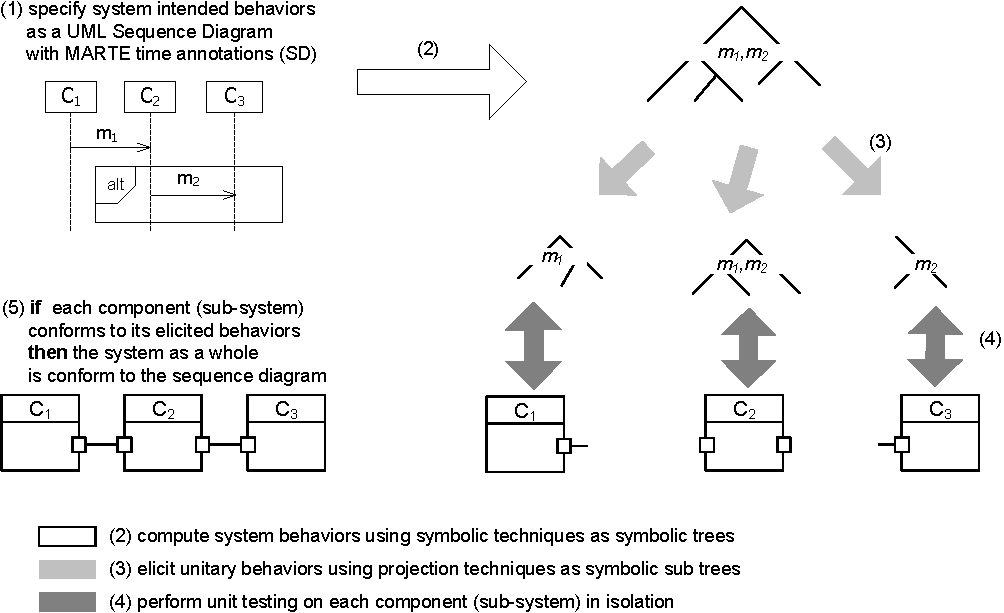
\includegraphics[scale=0.525]{approach_3.pdf}
\caption{\label{ct}Compositionnal Testing}
\end{figure}








\section{Microsoft's Verifier for Concurrent C (VCC)}

VCC is a tool from Microsoft Research
to prove correctness of annotated concurrent C programs.
It was mainly developed to verify Microsoft's \emph{Hyper-V} hypervisor.
%
It supports an own annotation language providing
e.g.\ contracts, pre- and postconditions, and type invariants.
%
It uses the Boogie tool to generate proof obligations,
and the automatic prover Z3 to prove them.
%
If an obligation is violated, the Model Viewer tool can generate a
counter-example use case.
%
VCC is available for non-commercial use from \cite{vcc}.


\section{The Proof Assistants Coq and Isabelle}


{\em Coq} is an interactive theorem prover and proof checker,
developed at INRIA, and based on
higher-order logic and the natural deduction calculus.
%
It provides the formal language {\em Gallina}, in which
mathematical definitions can be expressed as well as
executable algorithms and theorems.
%
The supporting tool for tactics-based semi-interactive development of
proofs is available from \cite{coq}.
%

{\em Isabelle}, maintained at Cambridge University,
and its predecessor {\em HOL}\footnote{
        Higher Order Logic
},
are similar tactic-oriented interactive theorem provers.
%
Isabelle is available from \cite{isabelle}.
%
While Isabelle is not yet supported in the Frama-C environment,
Coq is.


\section{The Model Checker NuSMV}

{\em SMV}\footnote{
        Symbolic Model Verifier
}
has been the first model checker based on binary decision
diagrams.
%
{\em NuSMV} is a reimplementation by the Fondazione Bruno Kessler
that is in addition capable of
performing SAT-based model-checking.
%
It supports both
Linear Temporal Logic (LTL) and Computation Tree Logic (CTL).
%
NuSMV's source code is available under an LGPL license from
\cite{nusmv}.


\section{Formal Verification of Real-Time Aspects based on Timed Automata}
\label{sct:twt:descrTA}

%\textcolor{magenta}{===== Start TWT =====}

Verifying system properties involving time is difficult with
traditional model checking methods. Commonly used \emph{temporal
  logics}, such as LTL or CTL catch discrete and qualitative aspects
of time and allow to formulate properties such as\footnote{The
  prefixes are the corresponding linear time operators.}
\begin{itemize}
  \item[\bf X] At the next point in time a property holds.
  \item[\bf F] At some future point in time a property holds.
  \item[\bf G] Always/generally (now and at any future point in time)
    a property holds. 
  \item[\bf U] A property $p$ holds until a property $q$ holds.
\end{itemize}

While it is possible to state properties that must be satisfied at
individual (discrete) points in time, continuous and quantitative
aspects of time as in the safety requirement
\begin{quote}
``The delay between receiving an emergency message and the issuing of
a brake order is less than 1 second.''
\end{quote}
are a real challenge. The problem does not stem from discrete
vs. continuous time, as any physical realisation of a real-time system
is inherently discretised by its clock. Instead, an operator for
expressing arbitrary temporal quantities or differences is
missing. Thus, for LTL and a clock of 1 kHz, it would be required to
use the operator \textbf{X} 1000 times. This notation is rather
unhandy, as it enforces to express a functional property relative to a
particular system.


This lack of expressivity is not merely a matter of notation, i.e.,
LTL or CTL, but also of the underlying semantics. Before introducing a
better suited logic we will first consider a formalism that serves as
this logic's semantics -- namely \emph{timed automata}.

\paragraph{Timed Automata}

Timed automata \cite{Alur1994} are essentially finite automata
extended with a finite set of clocks that all proceed at the same
rate. Clocks may be individually reset to zero. Clock variables can be
part of constraint expressions that may be used as transition
guards. A transition can only be taken if its guard is
fulfilled. Similarly, it is possible to specify an invariant for a
state that must be satisfied when the automaton is in this
state. Thus, we can enforce time constraints for the runs of the
automaton.

\paragraph{An Example}
The timed automaton in Figure~\ref{fig:ta:emergency1} depicts an
automaton representing an over-simplified version of an OBU subsystem
processing emergency messages. It has three states, one clock $x$ and
three actions, \textit{emg\_msg} (reception of an emergency message),
\textit{proc\_msg} (processing the message, e.g. raising an alarm) and
\textit{brake} (issueing the brake order). Upon receiving an emergency
message the clock $x$ is reset. The \textit{proc\_msg}-transition is
guarded by the clock constraint $x<1$ preventing the transition to be
taken if $x\geq 1$. The same holds for the \textit{brake}-transition.

\begin{figure}
\begin{center}
\begin{tikzpicture}[node distance=1.3cm,bend angle=45,auto]
\node [state, initial] (s1) at (0,0) { wait };
\node [state] (s2) at (4,0) { rcvd };
\node [state] (s3) at (8,0) { prcd };
\path[->] (s1) edge node {$\mathit{emg\_msg}, x:=0$}(s2);
\path[->] (s2) edge node {$x<1, \mathit{proc\_msg}$}(s3); 
\path[->] (s3) edge [bend left] node {$x<1, \mathit{brake}$}(s1);
\end{tikzpicture}
\end{center}
\caption{First (faulty) version of a timed automaton for processing
  emergency messages} 
\label{fig:ta:emergency1}
\end{figure}

One might think that the automaton from Figure~\ref{fig:ta:emergency1}
thus fulfills the safety requirement stated above. Due to the
operational semantics of timed automata this is not true: a timed
automaton in a given state can either take a transition or wait for an
arbitrary amount of time. Thus, if automaton waits in state rcvd and
$x$ exceeds one second, the system will deadlock as the next
transition is guarded by the constraint $x<1$. A run of the automaton
that could serve as counterexample is, e.g.

$$(\mathrm{wait},0)\rightarrow(\mathrm{wait},0.5)\rightarrow(\mathrm{rcvd},0.5)\rightarrow(\mathrm{rcvd},2)\rightarrow\textrm{DEADLOCK}$$

A solution to this problem is to force the automaton to proceed by
placing \emph{progress} constraints on the states. This has been done
in Figure~\ref{fig:ta:emergency2}. The transition guards have been
omitted as they are not necessary anymore. Now the safety property
``The delay between receiving an emergency message and the issuing of
a brake order is less than 1 second.'' is fulfilled.

\begin{figure}
\begin{center}
\small
\begin{tikzpicture}[node distance=1.3cm,bend angle=45,auto]
\node [state, initial] (s1) at (0,0) { wait };
\node [state] (s2) at (4,0) { rcvd }; 
\node [state] (s3) at (8,0) { prcd };
\node at (4,-0.7) {$x<1$};
\node at (8,-0.7) {$x<1$};
\path[->] (s1) edge node {$\mathit{emg\_msg}, x:=0$}(s2);
\path[->] (s2) edge node {$\mathit{proc\_msg}$}(s3); 
\path[->] (s3) edge [bend left] node {$\mathit{brake}$}(s1);
\end{tikzpicture}
\end{center}
\caption{Corrected version of the timed automaton for processing
  emergency messages}
\label{fig:ta:emergency2}
\end{figure}

\paragraph{UPPAAL}

\textsc{Uppaal} is a tool for modelling and verifying timed automata
developed by the universities of Uppsala and Aalborg
\cite{UppaalTutorial04}. This toolkit is under constant development
and comes with an academic as well as a commercial licence. Moreover,
there is a comparably large body of literature featuring
\textsc{Uppaal}, providing introductory and industrial examples.

\textsc{Uppaal} extends timed automata with synchronisation enabling
concurrent, communicating automata representing different parts of a
system. In addition, variables other than clocks are supported making
the modelling language more powerful. The logic used for expressing
real-time properties is a subset of TCTL (Timed Computation Tree
Logic). Nesting of temporal operators is not supported leading to a
restriction in expressiveness.

\paragraph{From SysML/UML to Timed Automata}

Timed automata and statecharts in SysML/UML are both based on the
concept of finite automata. Thus, it seems reasonable to extract timed
automata from existing statecharts which is addressed in the
literature \cite{David2002, Knapp2002, Jensen2004}. In this way,
safety properties -- formalised as TCTL formulae -- can be verified in
an automated fashion for a given statechart. However, there remain
challenges:
\begin{itemize}
\item Translating hierarchical states to timed automata is not
  straight-forward and complicates matters significantly. If an
  hierarchical state-chart is flattened, structural information is
  lost and makes the timed automaton more difficult to read and
  understand. Thus, it is advisable to retain some kind of hierarchy,
  possibly by using synchronisation mechanisms.
\item Special statechart features, such as history nodes that have a
  partially undefined semantics according to the current SysML/UML
  standard \cite{fecher_29_2005}, introduce problems. As they are not
  used very often, they can possibly left out in a first iteration.
\end{itemize}

%\textcolor{magenta}{===== End TWT =====}

\chapter{Verification with Model-Based Simulation}
\label{sct:uro:systemc}

%\textcolor{magenta}{===== Start URO (first draft) =====}

This section addresses verification based on simulation. By building
an executable model of system components its real-time behaviour can
by analysed and evaluated before actually building the entire system.

\section{Modelling with SysML and SystemC}

Specifications in natural language are difficult to handle. Breaking
down an overall system description into small comprehensible parts
reduces complexity and eases interdisciplinary communication to be
more efficient in performing development tasks.

SysML, developed by the OMG (Object Management Group), is a simple but
powerful general-purpose graphical modeling language that does not
directly support executable models. However, there is a variety of
tools for code generation from UML/SysML, especially for the Eclipse
platform and the Papyrus framework that will be used in the project.

To enable model execution and especially real-time simulation it is
considered to generate semi-formal SystemC code from that abstract
SysML models. It has to be investigated whether the the SysML model
have to be adapted to a domain or language specific version. Concrete
analysis will show whether this is feasible.

SystemC is a C++ library providing an event-driven simulation
interface suitable for electronic system design at various abstraction
levels (from high level down to individual hardware components). It
enables a system designer to simulate concurrent processes. SystemC
processes can communicate in a simulated real-time environment, using
channels of different datatypes (all C++ types and user defined types
are supported). SystemC supports hardware and software synthesis (with
the corresponding tools). SystemC models are executable.

\section{Model execution and simulation}

The aim of the execution of an SystemC model is to ensure that the
working capacity (performance) of the underlying hardware system is
sufficient to meet the system requirements. It has to be analysed
which hardware resources will be needed for the OBU to avoid excessive
delays and to ensure adequate response times in critical situations.
Because of the integrated simulation enviroment, SystemC enables
scheduling analysis for average and worst-case conditions and provides
analyses of process resources for individual system functions.

In addition, by creating an executable system model from SysML or UML,
the (real time) behaviour of the system can be analysed which is not
feasible at the SysML level.

%\textcolor{magenta}{===== End URO =====}


